\documentclass[12pt,a4paper]{article}

%:------- VIETNAMESE + FONT:-------
\usepackage[utf8]{inputenc}
\usepackage[T5]{fontenc}
\usepackage[vietnamese,english]{babel}
\usepackage{lmodern}

%:------- PACKAGES:-------
\usepackage{graphicx}
\usepackage{geometry}
\usepackage{tikz}
\usepackage{array}
\usepackage{tabularx}
\usepackage{setspace}
\usepackage{titlesec}
\usepackage{amsmath}
\usepackage{ragged2e}
\usepackage{makecell}
\usepackage{xcolor}
\usepackage{fancyhdr}
\usepackage{lastpage}
\usepackage{listings}
\usepackage{float}
\usepackage{tocloft}

\setlength{\cftbeforesecskip}{2pt}
\setlength{\cftbeforesubsecskip}{0pt}
\setlength{\cftbeforesubsubsecskip}{0pt}

\lstdefinestyle{matlabstyle}{
    language=Matlab,  
}
%:------- PAGE SETUP:-------
% Left margin is larger for binding.
\geometry{
    top=2.5cm,
    bottom=2.5cm,
    left=3.5cm,
    right=2.0cm
}
%:------- COLORS:-------
\definecolor{hcmutblue}{RGB}{0,80,170}
\definecolor{codebg}{rgb}{0.97,0.97,0.97}
\definecolor{codegreen}{rgb}{0.0,0.45,0.0}
\definecolor{codepurple}{rgb}{0.45,0.0,0.55}
\definecolor{codeblue}{rgb}{0.0,0.0,0.60}
\definecolor{codegray}{rgb}{0.45,0.45,0.45}


\setstretch{1.4}

\lstdefinestyle{code}{
    language=Matlab,
    backgroundcolor=\color{codebg},
    commentstyle=\color{codegreen}\itshape,
    keywordstyle=\color{codeblue}\bfseries,
    numberstyle=\tiny\color{codegray},
    stringstyle=\color{codepurple},
    basicstyle=\ttfamily\scriptsize,
    breakatwhitespace=false,
    breaklines=true,
    captionpos=b,
    keepspaces=true,
    numbers=left,
    numbersep=6pt,
    showspaces=false,
    showstringspaces=false,
    tabsize=4,
    frame=single,
    rulecolor=\color{gray!50},
    xleftmargin=1.5em,
    framexleftmargin=1.5em,
}



%:------- HEADER AND FOOTER STYLE:-------
\setlength{\headheight}{38pt}
\setlength{\headsep}{18pt}
\setlength{\footskip}{35pt}
\setlength{\parindent}{0em}
\fancypagestyle{mainstyle}{
    \fancyhf{}

    % Header
    \fancyhead[L]{
        \begin{minipage}{0.95\textwidth}
            \raisebox{-0.35\height}{\includegraphics[width=1.05cm]{{logo bk.png}}}
            \hspace{0.15cm}
            \begin{minipage}[b]{12cm}
                {\scriptsize\bfseries\textcolor{hcmutblue}{VIETNAM NATIONAL UNIVERSITY HO CHI MINH CITY}}\\[-1pt]
                {\scriptsize\bfseries\textcolor{hcmutblue}{HO CHI MINH CITY UNIVERSITY OF TECHNOLOGY}}
            \end{minipage}
        \end{minipage}
    }

    % Footer
    \fancyfoot[L]{
        \begin{minipage}{0.7\textwidth}
            {\scriptsize\bfseries Major Assignment Report Linear Algebra}\\[-1pt]
            {\scriptsize\bfseries Academic Year 2025--2026}
        \end{minipage}
    }

    \fancyfoot[R]{
        {\scriptsize\bfseries Page \thepage/\pageref{LastPage}}
    }

    \renewcommand{\headrulewidth}{0.6pt}
    \renewcommand{\footrulewidth}{0.6pt}
}

%:------- BORDER COMMAND FOR COVER:-------
\newcommand{\coverborder}{
\begin{tikzpicture}[remember picture, overlay]

    \draw[line width=0.7pt]
        ([xshift=1.45cm,yshift=-1.45cm]current page.north west)
        rectangle
        ([xshift=-1.45cm,yshift=1.45cm]current page.south east);

    \draw[hcmutblue,line width=1.6pt]
        ([xshift=1.70cm,yshift=-1.70cm]current page.north west)
        rectangle
        ([xshift=-1.70cm,yshift=1.70cm]current page.south east);

    \draw[line width=0.6pt]
        ([xshift=1.95cm,yshift=-1.95cm]current page.north west)
        rectangle
        ([xshift=-1.95cm,yshift=1.95cm]current page.south east);

    % Corner squares
    \draw[line width=0.5pt]
        ([xshift=1.32cm,yshift=-1.32cm]current page.north west)
        rectangle ++(0.32cm,-0.32cm);

    \draw[line width=0.5pt]
        ([xshift=-1.64cm,yshift=-1.32cm]current page.north east)
        rectangle ++(0.32cm,-0.32cm);

    \draw[line width=0.5pt]
        ([xshift=1.32cm,yshift=1.64cm]current page.south west)
        rectangle ++(0.32cm,-0.32cm);

    \draw[line width=0.5pt]
        ([xshift=-1.64cm,yshift=1.64cm]current page.south east)
        rectangle ++(0.32cm,-0.32cm);

\end{tikzpicture}
}

\begin{document}

% =====================================================
% PAGE 1: COVER PAGE
% =====================================================
\begin{titlepage}
\thispagestyle{empty}
\coverborder

\begin{center}

\vspace*{-0.25cm}

{\large\bfseries VIETNAM NATIONAL UNIVERSITY, HO CHI MINH CITY}\\[0.10cm]
{\large\bfseries HO CHI MINH CITY UNIVERSITY OF TECHNOLOGY}

\vspace{1.15cm}

\includegraphics[width=0.30\textwidth]{{logo bk.png}}

\vspace{1.10cm}

{\Large\bfseries LINEAR ALGEBRA PROJECT REPORT}

\vspace{0.55cm}

{\LARGE\bfseries GAME THEORY}

\vspace{0.95cm}

\begin{tabular}{>{\bfseries}r @{\hspace{0.35cm}} l}
Course:     & \bfseries LINEAR ALGEBRA \\
Instructor: & \bfseries Dang Thi Kim Nhung \\
Group:      & \bfseries 15b \\
Class:      & \bfseries CC02 \\
\end{tabular}

\vspace{1.25cm}

\renewcommand{\arraystretch}{1.18}
\setlength{\tabcolsep}{7pt}

\small
\begin{tabular}{|>{\centering\arraybackslash}p{6.3cm}
                |>{\centering\arraybackslash}p{4.3cm}|}
\hline
\textbf{Student Name} & \textbf{Student ID} \\
\hline
Phan Gia Kiệt &  2551131 \\
\hline
Nguyễn Phương Tâm Anh & 2551118 \\
\hline
Nguyễn Trần Hoàng Lan & 2551134 \\
\hline
Lê Trần Thục Khuê & 2551173 \\
\hline
Trần Thu Hiền & 2551126 \\
\hline
Đào Xuân Quang & 2551144 \\
\hline
\end{tabular}
\normalsize

\vfill

{\bfseries Ho Chi Minh City,  19 / May / 2026}

\vspace*{0.25cm}

\end{center}
\end{titlepage}

% Turn on header and footer from page 2 onward
\pagestyle{mainstyle}

% =====================================================
% PAGE 2: ASSIGNMENT SHEET
% =====================================================
\newpage
\vspace{0.5cm}

\begin{center}
    {\LARGE\bfseries ASSIGNMENT SHEET}
\end{center}

\vspace{0.3cm}
\renewcommand{\arraystretch}{1.6}
\setlength{\tabcolsep}{3pt}
%===============================================
%bảng
%===============================================
\renewcommand{\tabularxcolumn}[1]{m{#1}}
\renewcommand{\tabularxcolumn}[1]{m{#1}}

\begin{center}
\begin{tabularx}{\textwidth}{|
>{\centering\arraybackslash}m{2.5cm}|
>{\centering\arraybackslash}m{2.0cm}|
>{\centering\arraybackslash}X|
>{\centering\arraybackslash}m{2.5cm}|
>{\centering\arraybackslash}m{2.0cm}|}
\hline

\textbf{Full Name} 
& \textbf{Student ID} 
& \textbf{Assigned Tasks} 
& \textbf{Completion Rate}
& \textbf{Signature} \\
\hline

Phan Gia Kiệt 
& 2551131 
& \makecell[c]{Final checking\\Application scenarios 1, 2, 3\\Algorithm design}
& 100\% 
& 
\includegraphics[width=2cm]{s1.png}\\ 
\hline

Đào Xuân Quang
& 2551144 
& \makecell[c]{Algorithm design\\MATLAB implementation\\Technical description}
& 100\% 
& 
\includegraphics[width=2cm]{s2.png} \\
\hline

Nguyễn Trần Hoàng Lan 
& 2551134 
& Theoretical background
& 50\% 
& 
\includegraphics[width=2cm]{s3.png} \\
\hline

Lê Trần Thục Khuê 
& 2551173 
& Application scenario 1 
& 45\% 
& 
\includegraphics[width=2cm]{s4.png}\\
\hline

Nguyễn Thu Hiền 
& 2551126 
& Theoretical background 
& 49\% 
& 
\includegraphics[width=2cm]{s5.png}\\
\hline

Nguyễn Phương Tâm Anh 
& 2551118 
& Application scenario 2 
& 100\% 
& 
\includegraphics[width=2cm]{s6.png}\\
\hline

\end{tabularx}
\end{center}


\setlength{\tabcolsep}{6pt}


\begin{flushright}
\begin{tabular}{c}
\textbf{Team Leader's Confirmation} \\[0.2cm]

\includegraphics[width=3.5cm]{s1.png} \\[-0cm]
\makebox[5cm]{\hrulefill} \\[0.2cm]
\textbf{Phan Gia Kiệt}
\end{tabular}
\end{flushright}



%=======
% table of ct
%-------
\newpage

\begingroup
\small
\setstretch{1.4}
\tableofcontents
\endgroup
% =====================================================
% PAGE 6: INTRODUCTION
% =====================================================
\newpage


\section{Introduction}
\subsection{Motivation}
The study of strategic decision making has become very important in modern mathematics, and in many real world situations, individuals, companies, organizations must make decisions while considering the possible actions of their opponents. 

Matrix game theory, specifically two-player zero-sum games, provides the ability to analyzing competitive situations and determine optimal strategies. In practice, matrix games have applications in economics, business competition, etc,.. where strategic interaction are significant factors. 

This project aims to analyze strategic problems through matrix games and demonstrate how mathematical optimization methods can be used to determine effective strategies in real-world situations.


\subsection{Objectives of the Project}

The project was conducted to study and present the applications of matrices in game theory, specifically focusing on two-player zero-sum games. 

First, we focus on analyzing the main concepts such as pure strategy, mixed strategy, saddle point, and the minimax theorem. Also, we aim to explain the mathematical relationship between matrix games and linear programming through the construction of Linear Programming (LP) models. 

Second, the group will explain the algorithms used to solve matrix games for both the (2 × 2) case and general case, using Matlab to determine the optimal strategies and the value of the game. 

Finally, we apply game theory to real-world situations and analyze the economic and social significance of optimal strategies.


\subsection{Scope of the Study}

The scope of this project is limited to finite matrix games between two players with zero-sum payoffs.  

From an algorithmic perspective, the project focuses on studying methods for solving matrix games through linear programming and applying optimization algorithms to determine the optimal solutions. And to ensure a balance between theory and practical application, these methods will be applied to analyze three real world applicants in the socioeconomic field.

Finally, topics such as games with incomplete information, multiplayer games, cooperative games, and dynamic game models over time are beyond the scope of this project.



\section{Theoretical Background}
\subsection{Concept of Matrix Games: Two-Player Zero-Sum Games}

Matrix games are mathematical models used to analyze competitive situations between players with conflicting interests. In this model, the outcome is represented by a payoff matrix, where each element \(a_{ij}\) shows the payoff obtained when the first player chooses row strategy \(i\) and the second player chooses column strategy \(j\).

In this project, we focus on finite two-player zero-sum games. In this type of game, the total payoff of the two players is always zero, meaning that the gain of one player is exactly the loss of the other. Therefore, the first player aims to maximize their payoff, while the second player aims to minimize it \cite{osborne2004}.

The rows of the matrix usually represent the strategies of the first player, while the columns represent the strategies of the second player. A positive value of \(a_{ij}\) indicates an advantage for the first player, whereas a negative value indicates a disadvantage. Matrix games are widely applied in economics, military strategy, and social situations where decision makers must choose optimal strategies under competition and uncertainty.

\subsection{Pure Strategies and Mixed Strategies}

A strategy is a possible course of action that a player can choose in a game. In matrix games, there are two common types of strategies: pure strategies and mixed strategies.

A pure strategy means that a player always chooses one fixed action. It is simple and easy to analyze, but it can also make the player's behavior predictable and exploitable by the opponent. A mixed strategy means that a player chooses among several actions according to assigned probabilities. This helps reduce predictability, since the player does not always repeat the same action. Each probability must be non-negative, and the total probability must be equal to 1.

A mixed strategy of Player A can be represented as a probability vector over all available pure strategies. Suppose Player A has (n) strategies. Then the mixed strategy is given by

\noindent\makebox[\linewidth][c]{\(\displaystyle x = (x_1, x_2, \dots, x_n)^T\)}

where \(x_i\) denotes the probability that Player A chooses strategy (i). Therefore, the probabilities must satisfy

\noindent\makebox[\linewidth][c]{\(\displaystyle \ x_i \ge 0, \quad \sum_{i=1}^{n} x_i = 1 \)} 

\vspace{0.1CM}
This means that each strategy is assigned a non-negative probability, and the total probability over all strategies must be equal to one \cite{karlin1959}.


\subsection{Saddle Point}

A saddle point is an important concept in matrix games, used to determine whether a game has an optimal pure strategy solution.

To determine a saddle point, two values are commonly used: \(\max_i \min_j a_{ij})\) and \((\min_j \max_i a_{ij})\). Respectively, these values are called the maximin value and the minimax value.

Maximin is the strategy principle of Player A, who aims to maximize the minimum payoff that can be guaranteed. It is found by taking the minimum value of each row and then choosing the largest value among them.

Minimax is the strategy principle of Player B, who aims to minimize the maximum possible payoff of Player A. It is found by taking the maximum value of each column and then choosing the smallest value among them.

If the maximin value and the minimax value are equal, the game has a saddle point. This value is called the value of the game and also the value of the saddle point. In this case, the saddle point represents a stable solution for both players: Player A can guarantee a safe minimum payoff regardless of Player B's choice, while Player B can limit the maximum payoff that Player A may obtain. Therefore, neither player has an incentive to deviate from the corresponding pure strategy solution \cite{murthy2007}.


\textbf{Example:}

Given the following matrix:

\begingroup
\small
\renewcommand{\arraystretch}{0.75}
\setlength{\arraycolsep}{4pt}
\[
\begin{array}{c|cc}
 & B1 & B2\\
\hline
A1 & 3 & 1 \\
A2 & 5 & 2
\end{array}
\]
\endgroup

Consider each row: 

\noindent\makebox[\linewidth][c]{\(\displaystyle \min(A1)=1,\ \min(A2)=2, \ \max(1,2)=2\ \)}

\noindent\makebox[\linewidth][c]{\(\displaystyle \Rightarrow \text{maximin}=2  \)}


Consider each column: 

\noindent\makebox[\linewidth][c]{\(\displaystyle \max(B1)=5, \ \max(B2)=2,\ \min(5,2)=2\)}

\noindent\makebox[\linewidth][c]{\(\displaystyle \Rightarrow \text{minimax}=2\)}


Because maximin = minimax, the matrix above has a saddle point with value 2.

Saddle points help simplify the analysis of games because players do not need to use probabilities to choose strategies.




\subsection{Minimax Theorem}

The Minimax Theorem is one of the fundamental results in game theory. Introduced by John von Neumann in 1928, it plays a central role in the analysis of finite two-player zero-sum games \cite{thie2008}.

In this type of game, if a saddle point exists, both players can use pure strategies to reach the optimal result. However, many games do not have a saddle point, so using a fixed pure strategy may become predictable and exploitable. Therefore, mixed strategies are needed. Instead of always choosing one fixed action, each player assigns probabilities to their available strategies.

Suppose \(A\) is an \(m \times n\) payoff matrix, where Player A has \(m\) strategies and Player B has \(n\) strategies. Let \(x\) be the mixed strategy vector of Player A and \(y\) be the mixed strategy vector of Player B. The Minimax Theorem states that every finite two-player zero-sum game has a pair of optimal mixed strategies such that

\[
\max_x \min_y x^T A y = \min_y \max_x x^T A y = v
\]

Where \(v\) is the value of the game \cite{thie2008}.

To understand this formula more clearly, each component should be interpreted separately.  The vector \(x\) represents the mixed strategy of Player A, and \(x^T\) is the transpose of \(x\), while \(y\) represents the mixed strategy of Player B. Both of them are probability vectors, which means their elements are non-negative and the sum of their elements is equal to one. 

The expression \(x^T A y\) represents the expected payoff received by Player A when Player A uses the mixed strategy \(x\) and Player B uses the mixed strategy \(y\).

The left-hand side, \(\max_x \min_y x^T A y\), represents Player A's perspective. Player B is assumed to choose a mixed strategy \(y\) that minimizes Player A's expected payoff when Player A uses a given strategy \(x\), which is represented by \(\min_y x^T A y\). Therefore, Player A chooses the strategy \(x\) that makes this minimum payoff value as large as possible, represented by \(\max_x\).

The right-hand side, \(\min_y \max_x x^T A y\), represents Player B's perspective. Player A is assumed to choose a mixed strategy \(x\) that maximizes their expected payoff when Player B uses a given strategy \(y\), which is represented by \(\max_x x^T A y\). Therefore, Player B chooses the strategy \(y\) that makes this maximum payoff as small as possible, represented by \(\min_y\).

The equality of these two values means that the maximum payoff Player A can guarantee is exactly equal to the minimum upper bound that Player B can impose on Player A's payoff. This value is denoted by \(v\), and it is also called the value of the game.

The Minimax Theorem is not only important in game theory, but also has a close relationship with linear programming and modern optimization algorithms. This is also the mathematical foundation for building the matrix game solving program in this project.



\section{Mathematical Model and Algorithm}
\subsection{Relationship Between Matrix Games and Linear Programming}
In matrix game theory, the problem of finding optimal strategies has a close relationship with Linear Programming (LP). This relationship originates directly from the Minimax Theorem. However, most real-world problems do not have a saddle point, so players must use mixed strategies, represented by the probability vectors \(x\) and \(y\), such that:

\noindent\makebox[\linewidth][c]{\(\displaystyle x_i \ge 0 \quad \text{and} \quad y_j \ge 0 \)}

and 

\noindent\makebox[\linewidth][c]{\(\displaystyle\sum x_i = 1 \quad \text{and} \quad \sum y_j = 1 \)}

These probability conditions are linear constraints. Therefore, the problem of finding optimal strategies can be formulated as a Linear Programming problem \cite{thie2008}.

The objective of both players is to optimize the value of the game \(v\), which is determined by the expected payoff function. For Player A, the objective is to find the strategy vector \(x\) to maximize \(v\) (Maximin) and for Player B, the objective is to find the strategy vector \(y\) to minimize \(v\) (Minimax).

The transformation into a linear programming problem allows us to apply optimization methods such as the Simplex algorithm or built-in solver functions in Matlab to solve larger matrix game problems efficiently in practice.

\subsection{Equivalent Linear Programming Formulation}

\subsubsection{Payoff Matrix Shifting}

Assume the game is represented by the payoff matrix:

\noindent\makebox[\linewidth][c]{\(\displaystyle A=(a_{ij}) \)}

where  \(a_{ij}\) represents the payoff received by Player A when:

- Player A chooses row strategy \(i\)

- Player B chooses column strategy \(j\).




In practice, the payoff matrix may contain negative values. This creates difficulties when transforming the problem into a Linear Programming (LP) model, especially in later variable transformations involving division by the game value \(v'\).

To fix this issue, a positive constant \(c\) is added to every element of the matrix so that the smallest value in the matrix becomes positive:

\noindent\makebox[\linewidth][c]{\(\displaystyle a'_{ij}=a_{ij}+c \)}


The purposes of this transformation is to ensure all elements of the new matrix are positive, improving numerical stability during optimization, avoiding division by zero or negative values.

After the transformation, the new matrix becomes:


\noindent\makebox[\linewidth][c]{\(\displaystyle A'=(a'_{ij}) \)}

Also, adding the same constant to all payoff values does not change the optimal strategies of the players because every payoff increases equally. Only the value of the game changes:

\noindent\makebox[\linewidth][c]{\(\displaystyle v'=v+c \)}

where:

- original game value

- added positive constant

- shifted game value

After solving, the original game value will be recovered by:

\noindent\makebox[\linewidth][c]{\(\displaystyle v=v'-c \)  \cite{murthy2007}}
\subsubsection{Linear Programming Model for Player A}

Player A must determine the mixed strategy vector:

\noindent\makebox[\linewidth][c]{\(\displaystyle x=(x_1,x_2,\dots,x_m)^T \)}
where:

- is the probability of choosing row strategy \(i\)

- \(x_i \ge 0\)

The probability distribution must satisfy:
\vspace{0.1cm}

\noindent\makebox[\linewidth][c]{\(\displaystyle \sum_{i=1}^{m}x_i=1 \)}

\vspace{0.1cm}
According to the Maximin principle, Player A aims to maximize the minimum payoff that can be guaranteed.

More specifically, let \(v'\) denote the shifted game value. Then, regardless of which column strategy Player B chooses, the expected payoff of Player A must not be smaller than \(v'\).

This produces the constraint system:
\vspace{0.1cm}

\noindent\makebox[\linewidth][c]{\(\displaystyle  \sum_{i=1}^{m}a'_{ij}x_i \ge v'
\quad \forall j=1,\dots,n \)}

where:

- \(a'_{ij}\): payoff at row \(i\), column \(j\)

- \(x_i\): probability that Player A chooses row \(i\)

- \(\sum a'_{ij}x_i\): expected payoff of Player A if Player B selects column \(j\).

The objective is to maximize \( v'\). However, in this form, the variable \(v'\) appears throughout the constraint system, making it difficult to transform the problem into standard LP form.

Therefore, the following variable substitution is introduced:

\noindent\makebox[\linewidth][c]{\(\displaystyle X_i=\frac{x_i}{v'} \)}

This transformation eliminates the direct dependence on \(v'\) and converts the Maximin problem into a simpler linear inequality system. \cite{thie2008}

After substitution, the problem becomes:

\noindent\makebox[\linewidth][c]{\(\displaystyle \text{Minimize } \sum_{i=1}^{m}X_i \)}


subject to:

\noindent\makebox[\linewidth][c]{\(\displaystyle \sum_{i=1}^{m}a'_{ij}X_i \ge 1 \)} 

\vspace{0.1cm}
The transformation from ``maximize \(v'\)'' to ``minimize \(\sum X_i\)'' is derived as follows.

From:

\noindent\makebox[\linewidth][c]{\(\displaystyle X_i=\frac{x_i}{v'} \)}

we obtain:

\noindent\makebox[\linewidth][c]{\(\displaystyle x_i=v'X_i \)}


Substituting into the probability normalization condition:

\noindent\makebox[\linewidth][c]{\(\displaystyle \sum_{i=1}^{m}x_i=1\)}

gives:

\noindent\makebox[\linewidth][c]{\(\displaystyle v'\sum_{i=1}^{m}X_i=1\)}

Therefore:

\noindent\makebox[\linewidth][c]{\(\displaystyle \sum_{i=1}^{m}X_i=\frac1{v'}\)}

\vspace{0.1cm}
This means that when \(v'\) increases, \(\frac1{v'}\) decreases. Hence:

\noindent\makebox[\linewidth][c]{\(\displaystyle \max(v') \iff \min\left(\frac1{v'}\right)\)}

and since:

\noindent\makebox[\linewidth][c]{\(\displaystyle \frac1{v'}=\sum X_i\)}

the problem becomes equivalent to minimizing:

\noindent\makebox[\linewidth][c]{\(\displaystyle \sum X_i\)}

After solving the LP model, the optimal mixed strategy of Player A is recovered by normalization:

\noindent\makebox[\linewidth][c]{\(\displaystyle x_i=
\frac{X_i}
{\sum_{k=1}^{m}X_k}\)}

The shifted game value is:

\noindent\makebox[\linewidth][c]{\(\displaystyle v'=
\frac1
{\sum_{i=1}^{m}X_i}\)}

and the original game value is:

\noindent\makebox[\linewidth][c]{\(\displaystyle v=v'-c\)}

\subsubsection{Linear Programming Model for Player B}

Similarly, Player B constructs the mixed strategy vector:

\noindent\makebox[\linewidth][c]{\(\displaystyle y=(y_1,y_2,\dots,y_n)^T\)}

where:
\begin{itemize}
    \item \(y_j\) is the probability of choosing column strategy \(j\),
    \item \(y_j \ge 0\),
    \item the probabilities sum to 1.
\end{itemize}
Unlike Player A, Player B aims to minimize Player A’s payoff according to the Minimax principle.

Therefore, Player B must ensure that regardless of which row Player A selects, the expected payoff of Player A does not exceed a certain limit.

This leads to:

\noindent\makebox[\linewidth][c]{\(\displaystyle \sum_{j=1}^{n}a'_{ij}y_j \le v'\)}

where:

\noindent\makebox[\linewidth][c]{\(\displaystyle \sum a'_{ij}y_j\)}

represents the expected payoff of Player A when Player A selects row \(i\).

Similar to Player A’s formulation, a variable transformation is applied. 

Define the transformed variables:

\noindent\makebox[\linewidth][c]{\(\displaystyle Y_j=\frac{y_j}{v'}\)}

\vspace{0.1cm}
After substitution, the LP model for Player B becomes:
\vspace{0.1cm}

\noindent\makebox[\linewidth][c]{\(\displaystyle \text{Maximize } \sum_{j=1}^{n}Y_j\)}

subject to:

\noindent\makebox[\linewidth][c]{\(\displaystyle \sum_{j=1}^{n}a'_{ij}Y_j \le 1\) \cite{thie2008}} 

with:

\noindent\makebox[\linewidth][c]{\(\displaystyle Y_j \ge 0\)}

The transformation follows the same logic as Player A’s formulation. Since:
\vspace{0.1cm}

\noindent\makebox[\linewidth][c]{\(\displaystyle \sum_{j=1}^{n}y_j=1\)}

and:

\noindent\makebox[\linewidth][c]{\(\displaystyle y_j=v'Y_j\)}

we obtain:

\noindent\makebox[\linewidth][c]{\(\displaystyle v'\sum_{j=1}^{n}Y_j=1\)}

Therefore:

\noindent\makebox[\linewidth][c]{\(\displaystyle \sum_{j=1}^{n}Y_j=\frac1{v'}\)}

\vspace{0.1cm}
So, minimizing the upper bound \(v'\) is equivalent to maximizing:
\vspace{0.1cm}

\noindent\makebox[\linewidth][c]{\(\displaystyle \sum_{j=1}^{n}Y_j\)}

After solving the optimization system, the optimal mixed strategy probabilities of Player B are recovered by:

\noindent\makebox[\linewidth][c]{\(\displaystyle y_j=
\frac{Y_j}
{\sum_{k=1}^{n}Y_k}\)}

\vspace{0.15cm}
Through the Linear Programming formulation, the matrix game problem can be transformed into a linear optimization system that can be solved efficiently by computers, even for large matrices without saddle points.

\subsection{Algorithm for Solving 2$\times$2 Games and General Cases}

\subsubsection{General Structure of the Algorithm}

Given a payoff matrix \(A = (a_{ij})\), the algorithm starts by computing the minimum value of each row. Then, the maximin value is determined by choosing the largest value among the row minimum values. Similarly, the minimax value is determined by choosing the smallest value among the column maximum values.

After obtaining these two values, the algorithm compares the maximin and minimax values. If the maximin value is equal to the minimax value, then the game has a saddle point. In this case, the optimal solution is a pure strategy solution. Player A chooses the row containing the saddle point, while Player B chooses the column containing the saddle point. The value of the game is exactly equal to the payoff value at the saddle point.

Otherwise, if the maximin and minimax values are different, the game has no saddle point. In this situation, pure strategies are not sufficient to guarantee an optimal result. Therefore, mixed strategies must be used \cite{murthy2007}. 

\subsubsection{Algorithm for Solving 2x2 Matrix Games}

A two-player zero-sum game in which each player has two strategies can be represented by the following payoff matrix:

\begingroup
\small
\renewcommand{\arraystretch}{0.75}
\setlength{\arraycolsep}{4pt}
\[
\begin{array}{c|cc}
 & B1 & B2\\
\hline
A1 & a & b \\
A2 & c & d
\end{array}
\]
\endgroup

In this matrix, the rows represent the strategies of Player A, while the columns represent the strategies of Player B. For a \(2 \times 2\) game, the algorithm first checks whether a saddle point exists by comparing the maximin and minimax values. If a saddle point exists, the optimal pure strategies and the value of the game can be determined directly. If no saddle point exists, both players need to use mixed strategies.

Assume that Player A chooses the first row with probability p and the second row with probability 1-p. Player A chooses p so that Player B becomes indifferent between choosing the first column and the second column:

\noindent\makebox[\linewidth][c]{\(\displaystyle pa + (1-p)c = pb + (1-p)d \)}

Solving this equation gives:

\noindent\makebox[\linewidth][c]{\(\displaystyle p = \frac{d-c}{a-b-c+d} \)}

\vspace{0.15cm}
Therefore, the mixed strategy of Player A is:
\vspace{0.15cm}

\noindent\makebox[\linewidth][c]{\(\displaystyle  
x =
\begingroup
\renewcommand{\arraystretch}{0.7}
\begin{bmatrix}
p \\
1-p
\end{bmatrix}
\endgroup
\)}

\vspace{0.15cm}
Similarly, assume that Player B chooses the first column with probability \(q\) and the second column with probability \(1-q\). Player B chooses \(q\) so that Player A becomes indifferent between choosing the first row and the second row:

\noindent\makebox[\linewidth][c]{\(\displaystyle qa + (1-q)b = qc + (1-q)d\)}

Solving this equation gives:

\noindent\makebox[\linewidth][c]{\(\displaystyle q = \frac{d-b}{a-b-c+d}\)}

\vspace{0.15cm}
Therefore, the mixed strategy of Player B is:
\vspace{0.1cm}

\noindent\makebox[\linewidth][c]{\(\displaystyle 
y =
\begingroup
\renewcommand{\arraystretch}{0.7}
\begin{bmatrix}
q \\
1-q
\end{bmatrix}
\endgroup
\)}

The value of the game can be computed by:

\noindent\makebox[\linewidth][c]{\(\displaystyle v = x^T A y \)}

For the \(2 \times 2\) case, this value can also be calculated directly using the formula:
\vspace{0.1cm}

\noindent\makebox[\linewidth][c]{\(\displaystyle v = \frac{ad-bc}{a-b-c+d} \)   \cite{thie2008}}


\subsubsection{Algorithm for General M x N Matrix Games}

The direct formula used for the 2x2 case is not suitable for matrix games with larger dimensions. Therefore, Linear Programming is required. In the general case, Player A may have m strategies and Player B may have n strategies. The payoff matrix can be written as:

\noindent\makebox[\linewidth][c]{\(\displaystyle A = (a_{ij})_{m \times n} \)}

The general algorithm still follows the same initial structure as the 2x2 case. First, the minimum value of each row, the maximum value of each column, the maximin value, and the minimax value are computed. Then, the algorithm checks whether the game has a saddle point.

If the maximin value is equal to the minimax value, the game has a saddle point and can be solved using pure strategies. If the maximin value is different from the minimax value, the game has no saddle point. For a general \(m \times n\) game, the optimal mixed strategies are found using Linear Programming.

\section{Results, Deliverables, and Applications}
\subsection{Experimental Results as Real-World Applications}

\subsubsection{Net Profit Competition Between Two Companies}

Although microeconomic competition in real life is not always strictly zero-sum, this model simplifies the situation by focusing on the relative advantage between two companies within the same short-term business campaign.

In this scenario, we consider a competition between Company A and Company B in the same market area. Both companies sell similar products, but they have slightly different market positions. Company A has a slightly higher initial price than Company B because it focuses more on product quality and after-sales service. In each short-term campaign, both companies must choose one of two strategies: offering a deep discount (1) or maintaining the price while improving after-sales service (2).

The payoff matrix represents the relative net profit advantage of Company A compared with Company B in one campaign. A positive payoff means that Company A obtains a higher relative net profit advantage, while a negative payoff means that Company A performs worse. A payoff of zero does not mean that both companies break even; it only means that their relative net profit advantages are approximately balanced.

\begingroup
\small
\renewcommand{\arraystretch}{0.75}
\setlength{\arraycolsep}{4pt}
\[
\begin{array}{c|cc}
 & B1 & B2\\
\hline
A1 & -1 & -2 \\
A2 & 3 & 0
\end{array}
\]
\endgroup

When both companies offer deep discounts, the payoff is $-1$, showing that Company A is slightly disadvantaged because its original price is higher than Company B's. Even after discounting, Company A still suffers from higher promotional costs and a lower profit margin. If Company A discounts while Company B improves after-sales service, the payoff decreases to $-2$ because Company A loses profit from discounting and fails to use its quality-based positioning. On the other hand, if Company A improves after-sales service while Company B discounts, the payoff is $3$ because Company A can use its higher-quality brand image and maintain a better profit margin, while Company B sacrifices profit to compete on price. When both companies improve after-sales service, the payoff is $0$, representing a relative balance: Company A has the advantage of quality, while Company B has the advantage of lower price.

From the matrix, the minimum values of the two rows are $-2$ and $0$, so the maximin value is $0$. The maximum values of the two columns are $3$ and $0$, so the minimax value is also $0$. Since the maximin and minimax values are equal, the game has a saddle point at $(A2,B2)$. This means that the equilibrium strategy for both companies is to avoid a price war and focus on after-sales service in order to maintain stable net profit and avoid destructive price competition.

\subsubsection{Strategic Macroeconomic Competition Between Two Countries}

Although macroeconomic relations are not always strictly zero-sum in reality, this model simplifies the situation by considering the relative strategic advantage between two countries during each policy phase. In this scenario, Country A wants to expand its economic influence and improve its global position, while Country B wants to protect its existing socioeconomic pillars in order to maintain growth, employment, and social stability.

The competition takes place through economic tools such as tariffs, export controls, investment policies, and technology development. The economy is divided into three strategic areas. Alpha represents high technology and innovation; Bravo represents supply chains and industrial production; and Charlie represents consumer markets, social media influence, and soft power.

Each country can choose to focus on one area or combine two areas for attack or defense. If one area is chosen, resources are concentrated. If two areas are chosen, resources are divided. Therefore, each side has six strategies: Alpha, Bravo, Charlie, Alpha-Bravo, Alpha-Charlie, and Bravo-Charlie. Each round is understood as a policy decision phase, in which long-term effects such as supply chain changes and market sentiment are indirectly reflected in the payoff values.

The payoff matrix is calculated from the perspective of Country A. A positive value means that Country A gains a relative socioeconomic advantage over Country B, while a negative value means that Country A is disadvantaged. The payoff matrix is given by

\begingroup
\small
\renewcommand{\arraystretch}{0.75}
\setlength{\arraycolsep}{4pt}
\[
\begin{array}{c|cccccc}
 & B1 & B2 & B3 & B4 & B5 & B6 \\
\hline
A1 & -4 & 5 & 6 & -2 & -1 & 4 \\
A2 & 4 & -3 & 5 & -1 & 3 & 0 \\
A3 & 3 & 4 & -2 & 2 & -1 & -1 \\
A4 & 1 & 2 & 7 & 0 & 2 & 1 \\
A5 & 2 & 6 & 3 & 1 & 0 & 2 \\
A6 & 5 & 1 & 2 & 3 & 1 & 0
\end{array}
\]
\endgroup
In general, when Country A focuses on an area that Country B does not protect, the payoff is positive because A can exploit a policy gap and gain an advantage. Conversely, when Country B protects the same area that Country A attacks, the payoff is usually negative because A faces defensive measures such as industrial subsidies, export controls, supply chain reinforcement, or domestic market stabilization.

For combined strategies involving two areas, the payoff depends on how much the attack scope of Country A overlaps with the defense scope of Country B. If Country B leaves important pillars such as Alpha or Bravo unprotected, Country A can obtain a high payoff. If both countries allocate resources to corresponding areas, the payoff tends to move closer to $0$, representing a relative balance. Therefore, the matrix does not simply describe winning or losing, but also reflects the trade-off between policy effectiveness, resource dispersion, and the predictability of the opponent's actions.

The computational results show that the maximin value is $0$ and the minimax value is $3$, so the game has no saddle point. This means that neither country should use a fixed pure strategy, because the opponent can predict it and exploit the remaining policy gaps. The optimal mixed strategy of Country A is

\noindent\makebox[\linewidth][c]{\(\displaystyle x=[0,\ 0,\ 0,\ 0.4167,\ 0.3333,\ 0.25] \)}

This means that Country A should not focus on only one single area. Instead, it should prioritize combined strategies: Alpha-Bravo with probability $41.67\%$, Alpha-Charlie with probability $33.33\%$, and Bravo-Charlie with probability $25\%$. Alpha-Bravo has the highest probability because high technology and supply chains are the two most strategically valuable areas.

The optimal mixed strategy of Country B is

\noindent\makebox[\linewidth][c]{\(\displaystyle y=[0,\ 0,\ 0,\ 0.25,\ 0.3333,\ 0.4167] \)}


This means that Country B should also avoid defending only one fixed pillar. Instead, it should distribute its defensive resources among Alpha-Bravo, Alpha-Charlie, and Bravo-Charlie. The value of the game is

\noindent\makebox[\linewidth][c]{\(\displaystyle V=1.0833 \)}

This indicates that Country A has a slight long-term advantage if it allocates its policy resources properly. From an economic and social perspective, the model shows that an effective strategy is not to concentrate completely on one pillar, but to flexibly allocate resources among technology, supply chains, and social influence in order to optimize benefits and reduce policy risks.

\subsubsection{Sidewalk Encroachment Control in Urban Areas}

In this scenario, we consider a social conflict between Urban Management Authority A and informal street vendors B in a densely populated urban area. The authority wants to maintain public order, reduce congestion, and preserve urban hygiene, while the street vendors want to continue selling on the sidewalk in order to maximize their income. The game cycle is counted weekly, and each side cannot change its strategy until the end of the week.

Urban Management Authority A has three strategies. A1 is giving warnings and conducting one regular inspection per day. A2 is issuing fines and conducting continuous patrols by shifts throughout the day. A3 is coordinating multiple departments, conducting one large-scale weekly sweep, and imposing heavy fines. The informal vendors B have four strategies. B1 is temporary compliance, B2 is selling during low-inspection hours, B3 is leaving during inspection and returning afterward, and B4 is coordinating as a group to avoid inspection and frequently changing locations.

The payoff is calculated from the perspective of Urban Management Authority A. A positive value represents effective public-order control after subtracting operating costs. A negative value represents weak control, high cost, or successful avoidance by group B.

\begingroup
\small
\renewcommand{\arraystretch}{0.75}
\setlength{\arraycolsep}{4pt}
\[
\begin{array}{c|cccc}
 & B1 & B2 & B3 & B4 \\
\hline
A1 & 5 & -2 & -2 & -4 \\
A2 & 3 & 2 & 1 & -3 \\
A3 & -1 & -3 & -3 & 6
\end{array}
\]
\endgroup

When group B only complies temporarily, simple measures can still produce positive payoffs. However, using A3 in this case is inefficient because the cost of large-scale sweeps and heavy punishment is higher than necessary, resulting in a payoff of $-1$. When group B avoids inspection as an organized group and changes locations frequently, A1 and A2 perform poorly with negative payoffs, while A3 achieves a payoff of $6$ because a strong measure is more suitable for organized behavior. For intermediate behaviors such as selling during low-inspection hours or returning after inspection, A2 is a more balanced choice because it creates continuous pressure without being excessively costly.

From the matrix, the maximin value is $-3$ and the minimax value is $1$, so the game has no saddle point. Therefore, the authority should not use one fixed strategy, but should apply a mixed strategy: A2 with probability about $69.23\%$ and A3 with probability about $30.77\%$, while A1 should not be the main long-term strategy. Group B will mainly choose B3 with probability about $69.23\%$ and B4 with probability about $30.77\%$. The value of the game is approximately $-0.2308$, showing that sidewalk encroachment remains difficult to control if informal vendors continuously change their behavior.

Therefore, if the authority relies only on confrontational administrative measures such as inspections and sweeps, it will still face long-term difficulties. A deeper social solution is also needed, such as social support, better urban planning, and designated legal spaces for small vendors.

\subsection{Deliverables of the project}
\subsubsection{Source code}
\begin{lstlisting}[style=code]
function LN_AGB_GT()
clc; clear;
%% GraphicalUserInterface
fig=uifigure('Name','NxM Matrix Game Solver','Position',[100 100 1200 720]);
uilabel(fig,'Text','NxM Zero-Sum Matrix Game Solver','Position',[380 670 450 30],'FontSize',22,'FontWeight','bold');
%% MatrixSizeInput
uilabel(fig,'Text','Rows (Player A)','Position',[80 620 150 25],'FontSize',14); rowField=uieditfield(fig,'numeric','Position',[220 620 80 25],'Value',3);
uilabel(fig,'Text','Columns (Player B)','Position',[350 620 170 25],'FontSize',14); colField=uieditfield(fig,'numeric','Position',[540 620 80 25],'Value',3);
%% Buttons
uibutton(fig,'push','Text','Create Matrix','Position',[680 620 140 35],'FontSize',14,'ButtonPushedFcn',@(btn,event)createMatrix());
uibutton(fig,'push','Text','Solve Game','Position',[850 620 140 35],'FontSize',14,'ButtonPushedFcn',@(btn,event)solveGame());
uibutton(fig,'push','Text','Show Charts','Position',[1020 620 140 35],'FontSize',14,'ButtonPushedFcn',@(btn,event)showCharts());
%% MatrixInputTable
uilabel(fig,'Text','Enter Payoff Matrix A','Position',[470 560 250 30],'FontSize',18);
matrixTable=uitable(fig,'Data',zeros(3,3),'Position',[250 300 700 240],'ColumnEditable',true);
%% ResultDisplay
resultText=uitextarea(fig,'Position',[120 30 950 240],'FontSize',14);
%% StoreResult
currentResult=[];
%% CreateMatrixCallback
function createMatrix()
r=max(2,round(rowField.Value)); c=max(2,round(colField.Value));
if r<2||c<2,uialert(fig,'Matrix must be at least 2x2.','Invalid Size'); return; end
matrixTable.Data=zeros(r,c);
end
%% SolveCallback
function solveGame()
A=matrixTable.Data;
try
currentResult=mainGameSolver(A);
matrixRows=strings(size(A,1),1);
for i=1:size(A,1), matrixRows(i)="[ "+join(string(A(i,:))," ")+" ]"; end
matrixString=join(matrixRows,newline);
output=["========== GAME THEORY RESULTS ==========","","PAYOFF MATRIX:",matrixString,"","MAXIMIN VALUE = "+num2str(currentResult.maximin),"MINIMAX VALUE = "+num2str(currentResult.minimax),""];
if currentResult.hasSaddle
output=[output,"SADDLE POINT EXISTS","SADDLE POINT POSITION = (A"+num2str(currentResult.saddleRow)+", B"+num2str(currentResult.saddleCol)+")"];
else
output=[output,"NO SADDLE POINT"];
end
output=[output,"","PLAYER A MIXED STRATEGY:",mat2str(currentResult.strategyA,4),"","PLAYER B MIXED STRATEGY:",mat2str(currentResult.strategyB,4),"","VALUE OF THE GAME = "+num2str(currentResult.gameValue),"","EXPECTED PAYOFF xTransposeAy = "+num2str(currentResult.expectedValue)];
resultText.Value=output;
catch ME
resultText.Value=ME.message;
end
end
%% ChartCallBack
function showCharts()
if isempty(currentResult), uialert(fig,'Solve the game first.','No Data'); return; end
plotStrategies(currentResult);
end
end
%% SOLVER
function result=mainGameSolver(A)
%% ExtractMatrixSize
[m,n]=size(A);
%% SADDLEPOINT CALC
rowMin=min(A,[],2); maximin=max(rowMin);
colMax=max(A,[],1); minimax=min(colMax);
result.maximin=maximin; result.minimax=minimax;
%% SaddlePointChecker
tol=1e-8;
if abs(maximin-minimax)<tol
result.hasSaddle=true;
[r,c]=find(abs(A-maximin)<tol,1);
strategyA=zeros(m,1); strategyB=zeros(n,1);
strategyA(r)=1; strategyB(c)=1;
result.saddleRow=r; result.saddleCol=c;
result.strategyA=strategyA; result.strategyB=strategyB;
result.gameValue=maximin;
strategyATranspose=transpose(strategyA);
result.expectedValue=strategyATranspose*A*strategyB;
result.matrix=A; return;
else
result.hasSaddle=false; result.saddleRow=[]; result.saddleCol=[];
%% Algorithm Branching
if m==2&&n==2
%% 1. Algebraic formula for 2x2 games
a=A(1,1); b=A(1,2); c=A(2,1); d=A(2,2);
den=a-b-c+d;
if abs(den)<tol, error('Degenerate 2x2 game.'); end
p=(d-c)/den; q=(d-b)/den;
p=max(0,min(1,p)); q=max(0,min(1,q));
strategyA=[p;1-p];
strategyB=[q;1-q];
v=(a*d-b*c)/den;
else
%% 2. Linear programming for general m x n games
shift=abs(min(A(:)))+1;
A1=A+shift;
opt=optimoptions('linprog','Display','none');
fA=ones(m,1);
x=linprog(fA,-transpose(A1),-ones(n,1),[],[],zeros(m,1),[],opt);
if isempty(x), error('Unable to solve Player A strategy.'); end
valueA=1/sum(x);
strategyA=x*valueA;
fB=-ones(n,1);
y=linprog(fB,A1,ones(m,1),[],[],zeros(n,1),[],opt);
if isempty(y), error('Unable to solve Player B strategy.'); end
valueB=1/sum(y);
strategyB=y*valueB;
%% Game value
v=((valueA+valueB)/2)-shift;
end
%% Expected Payoff and Store Results
strategyATranspose=transpose(strategyA);
expectedValue=strategyATranspose*A*strategyB;
result.strategyA=strategyA;
result.strategyB=strategyB;
result.gameValue=v;
result.expectedValue=expectedValue;
result.matrix=A;
end
end
%% C H A R T
function plotStrategies(result)
figure('Name','Game Theory Charts','NumberTitle','off','Position',[100 100 1400 450]);
%% PlayerAStrat
subplot(1,3,1);
bar(result.strategyA);
title('Player A Strategy');
xlabel('Strategies');
ylabel('Probability');
ylim([0 1]);
grid on;
%% PlayerBStrat
subplot(1,3,2);
bar(result.strategyB);
title('Player B Strategy');
xlabel('Strategies');
ylabel('Probability');
ylim([0 1]);
grid on;
%% PayoffHeatmap
subplot(1,3,3);
imagesc(result.matrix);
colorbar;
title('Payoff Matrix Heatmap');
xlabel('Player B');
ylabel('Player A');
[m,n]=size(result.matrix);
set(gca,'XTick',1:n,'YTick',1:m);
textStrings=string(result.matrix(:));
[x,y]=meshgrid(1:n,1:m);
text(x(:),y(:),textStrings(:),'HorizontalAlignment','center','FontSize',12,'Color','white');
end
\end{lstlisting}

\subsubsection{Output Data}

\par\noindent\textbf{Application 1}

\medskip
\noindent\textbf{Input:}

\begingroup
\small
\renewcommand{\arraystretch}{0.75}
\setlength{\arraycolsep}{4pt}
\[
\begin{array}{c|cc}
 & B1 & B2\\
\hline
A1 & -1 & -2 \\
A2 & 3 & 0
\end{array}
\]
\endgroup

\noindent\textbf{Output:}

\begin{lstlisting}[style=code]
========== GAME THEORY RESULTS ==========
PAYOFF MATRIX:
[ -1 -2 ]
[ 3 0 ]
MAXIMIN VALUE = 0
MINIMAX VALUE = 0
SADDLE POINT EXISTS
SADDLE POINT POSITION = (A2, B2)
PLAYER A MIXED STRATEGY:[0;1]
PLAYER B MIXED STRATEGY:[0;1]
VALUE OF THE GAME = 0
EXPECTED PAYOFF x^T A y = 0
\end{lstlisting}

\begin{figure}[H]
    \centering
    \makebox[\linewidth][c]{%
        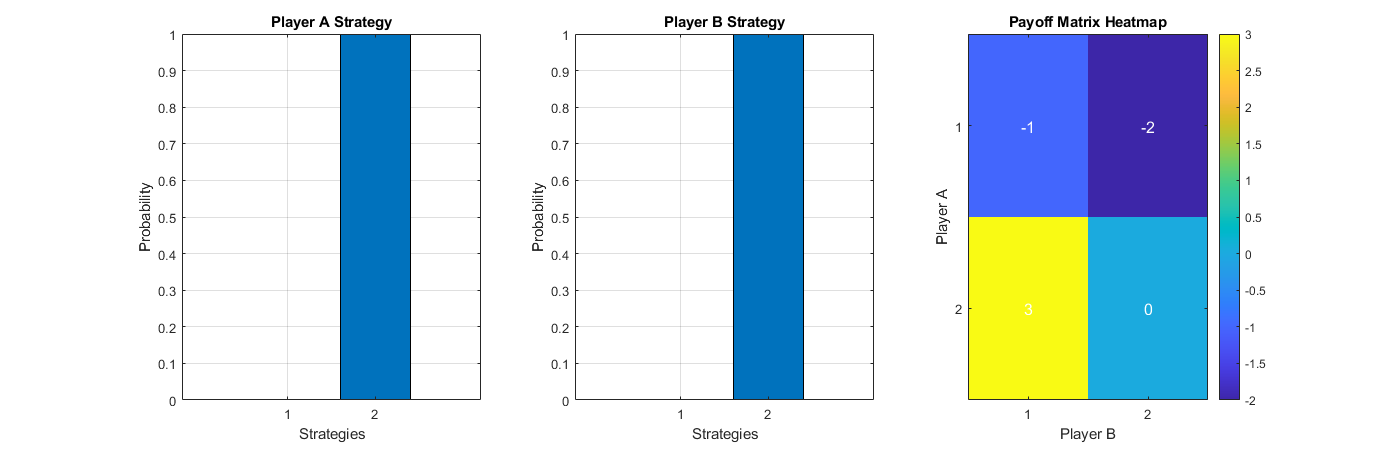
\includegraphics[width=1.35\linewidth]{1.png}
    }
    \caption{Graphical output for Application 1}
    \label{fig:application1-output}
\end{figure}


\par\noindent\textbf{Application 2}

\medskip
\noindent\textbf{Input:}

\begingroup
\small
\renewcommand{\arraystretch}{0.75}
\setlength{\arraycolsep}{4pt}
\[
\begin{array}{c|cccccc}
 & B1 & B2 & B3 & B4 & B5 & B6 \\
\hline
A1 & -4 & 5 & 6 & -2 & -1 & 4 \\
A2 & 4 & -3 & 5 & -1 & 3 & 0 \\
A3 & 3 & 4 & -2 & 2 & -1 & -1 \\
A4 & 1 & 2 & 7 & 0 & 2 & 1 \\
A5 & 2 & 6 & 3 & 1 & 0 & 2 \\
A6 & 5 & 1 & 2 & 3 & 1 & 0
\end{array}
\]
\endgroup

\noindent\textbf{Output:}

\begin{lstlisting}[style=code]
========== GAME THEORY RESULTS ==========
PAYOFF MATRIX:
[ -4 5 6 -2 -1 4 ]
[ 4 -3 5 -1 3 0 ]
[ 3 4 -2 2 -1 -1 ]
[ 1 2 7 0 2 1 ]
[ 2 6 3 1 0 2 ]
[ 5 1 2 3 1 0 ]
MAXIMIN VALUE = 0
MINIMAX VALUE = 3
NO SADDLE POINT
PLAYER A MIXED STRATEGY:[0;0;0;0.4167;0.3333;0.25]
PLAYER B MIXED STRATEGY:[0;0;0;0.25;0.3333;0.4167]
VALUE OF THE GAME = 1.0833
EXPECTED PAYOFF x^T A y = 1.0833
\end{lstlisting}

\begin{figure}[H]
    \centering
    \makebox[\linewidth][c]{%
        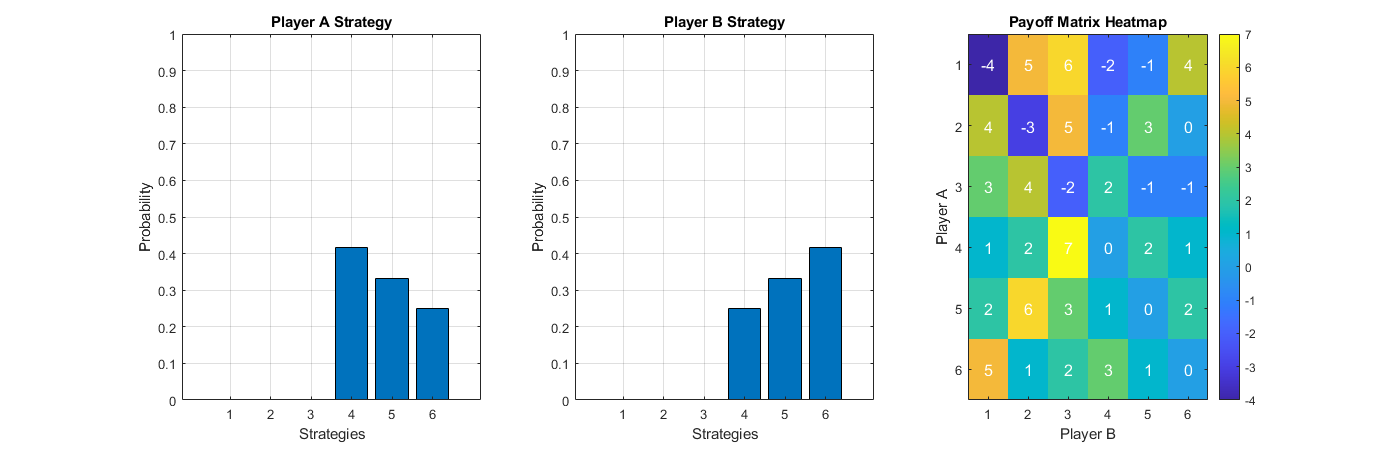
\includegraphics[width=1.35\linewidth]{2.png}
    }
    \caption{Graphical output for Application 2}
    \label{fig:application2-output}
\end{figure}


\par\noindent\textbf{Application 3}

\medskip
\noindent\textbf{Input:}

\begingroup
\small
\renewcommand{\arraystretch}{0.75}
\setlength{\arraycolsep}{4pt}
\[
\begin{array}{c|cccc}
 & B1 & B2 & B3 & B4 \\
\hline
A1 & 5 & -2 & -2 & -4 \\
A2 & 3 & 2 & 1 & -3 \\
A3 & -1 & -3 & -3 & 6
\end{array}
\]
\endgroup

\noindent\textbf{Output:}

\begin{lstlisting}[style=code]
========== GAME THEORY RESULTS ==========
PAYOFF MATRIX:
[ 5 -2 -2 -4 ]
[ 3 2 1 -3 ]
[ -1 -3 -3 6 ]
MAXIMIN VALUE = -3
MINIMAX VALUE = 1
NO SADDLE POINT
PLAYER A MIXED STRATEGY:[0;0.6923;0.3077]
PLAYER B MIXED STRATEGY:[0;0;0.6923;0.3077]
VALUE OF THE GAME = -0.23077
EXPECTED PAYOFF x^T A y = -0.23077
\end{lstlisting}

\begin{figure}[H]
    \centering
    \makebox[\linewidth][c]{%
        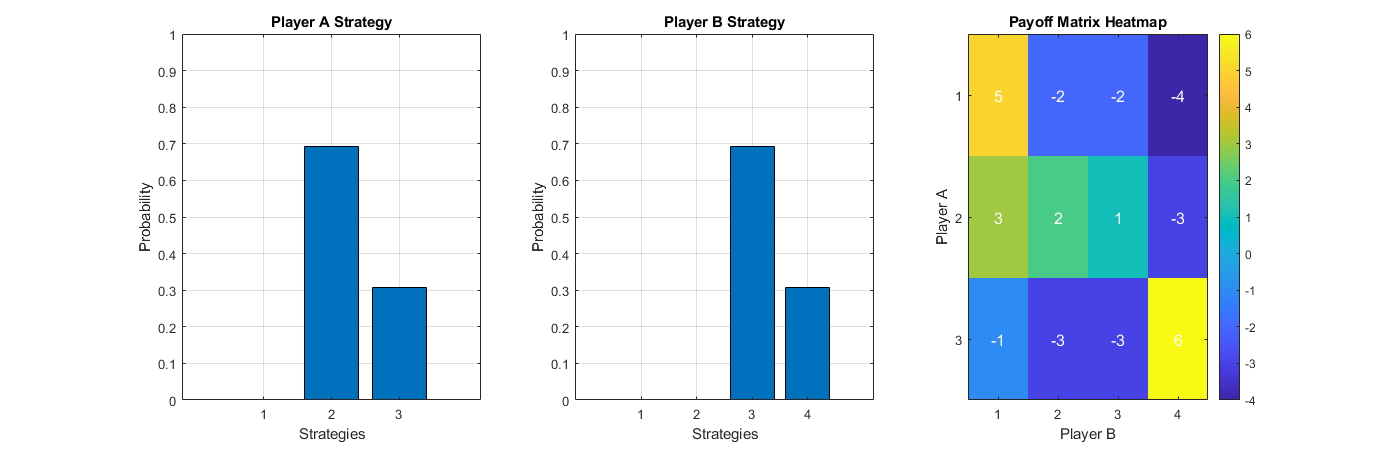
\includegraphics[width=1.35\linewidth]{3.png}
    }
    \caption{Graphical output for Application 3}
    \label{fig:application3-output}
\end{figure}
\subsection{Technical description}

The developed system is a MATLAB-based Graphical User Interface (GUI) application designed to solve \(N \times M\) zero-sum matrix games using classical game theory methods. The application allows users to create payoff matrices of varying dimensions, compute optimal strategies for both players, identify saddle points, calculate the value of the game, and visualize the results through graphical charts. The system combines numerical optimization, matrix computation, and interactive visualization into a single integrated application. It was implemented using MATLAB built-in GUI components and optimization libraries to provide an efficient and user-friendly environment for solving matrix games.
\paragraph{Programming Language Used:}

The programming language used in this project is MATLAB. It is used for numerical computation, matrix manipulation, GUI development, optimization, and data visualization.

\paragraph{Main Libraries and Built-in Functions:}

The application interface is constructed using MATLAB GUI components, including \texttt{uifigure}, \texttt{uibutton}, \texttt{uitable}, \texttt{uieditfield}, \texttt{uilabel}, and \texttt{uitextarea}. These components enable interactive data entry and result presentation. The mathematical solving process relies on MATLAB numerical computation tools such as \texttt{linprog}, \texttt{min}, \texttt{max}, \texttt{find}, \texttt{size}, \texttt{zeros}, and \texttt{abs}. These functions are used for saddle point detection, mixed strategy computation, linear programming optimization, and matrix analysis. The visualization module uses \texttt{bar}, \texttt{imagesc}, \texttt{subplot}, and \texttt{colorbar}. These functions help users analyze strategy distributions and payoff matrix structures.

\paragraph{Main GUI Function - \texttt{LNAGB\_SAMPLE\_6():}}

This is the primary controller function of the application. It initializes the GUI window, creates the application interface, accepts matrix dimensions from the user, generates editable payoff matrices, executes solving algorithms, displays textual results, and launches graphical visualizations. The interface contains input fields for the number of rows of Player A and the number of columns of Player B. It also includes three control buttons: \texttt{Create Matrix}, \texttt{Solve Game}, and \texttt{Show Charts}. The matrix input area is an editable payoff matrix table, while the output area displays the maximin value, minimax value, saddle point information, mixed strategies, expected payoff, and game value.

\paragraph{Matrix Creation Module - \texttt{createMatrix():}}

This callback function dynamically generates a payoff matrix according to user-defined dimensions. It reads the matrix dimensions from numeric input fields, validates the matrix size, creates a zero matrix, and updates the GUI table.

\begin{lstlisting}[style=code]
matrixTable.Data = zeros(rows,cols);
\end{lstlisting}

The system ensures that the matrix size is at least \(2 \times 2\). This prevents invalid game configurations.

\begin{lstlisting}[style=code]
uialert(fig,'Matrix must be at least 2x2.','Invalid Size');
\end{lstlisting}

\paragraph{Solver Module - \texttt{solveGame():}}

This module retrieves the payoff matrix entered by the user and executes the main solving algorithm. The matrix is retrieved from the GUI table as follows:

\begin{lstlisting}[style=code]
A = matrixTable.Data;
\end{lstlisting}

Then, the main solver is executed:

\begin{lstlisting}[style=code]
currentResult = mainGameSolver(A);
\end{lstlisting}

The module formats and displays the payoff matrix, maximin value, minimax value, saddle point status, mixed strategies, game value, and expected payoff. It also uses a \texttt{try-catch} structure to prevent application crashes caused by invalid matrix values, degenerate games, or optimization failures. This improves program stability and reliability.

\paragraph{Core Algorithm Module - \texttt{mainGameSolver(A):}}

This function contains the main game theory computations. The algorithm first computes the row minimums and column maximums:

\begin{lstlisting}[style=code]
rowMin = min(A,[],2);
colMax = max(A,[],1);
\end{lstlisting}

Then, the maximin and minimax values are computed:

\begin{lstlisting}[style=code]
maximin = max(rowMin);
minimax = min(colMax);
\end{lstlisting}

The program checks whether the difference between the maximin and minimax values is smaller than a tolerance value:

\noindent\makebox[\linewidth][c]{\(\displaystyle |maximin-minimax|<tol\)}

If this condition is true, the game contains a saddle point and pure strategies are assigned. Probability \(1\) is assigned to the optimal row and optimal column, while all other strategies receive probability \(0\). This produces deterministic optimal strategies.

\paragraph{2x2 Mixed Strategy Solver}

For non-saddle 2x2 games, the program uses direct algebraic formulas instead of linear programming. The mixed strategy probability for Player A is:

\noindent\makebox[\linewidth][c]{\(\displaystyle p=\frac{d-c}{a-b-c+d}\)}

The mixed strategy probability for Player B is:

\noindent\makebox[\linewidth][c]{\(\displaystyle q=\frac{d-b}{a-b-c+d}\)}

The value of the game is:

\noindent\makebox[\linewidth][c]{\(\displaystyle v=\frac{ad-bc}{a-b-c+d}\)} \cite{murthy2007}

This method provides fast computation, exact analytical solutions, and reduced computational cost for standard 2x2 games.

\paragraph{General \(N \times M\) Linear Programming Solver}

For larger matrices, the application applies linear programming optimization. To eliminate negative coefficients during optimization, the matrix is shifted:

\begin{lstlisting}[style=code]
shiftValue = abs(min(A(:))) + 1;
Ashift = A + shiftValue;
\end{lstlisting}

This guarantees positive constraint values.

For Player A, the optimization objective and constraints are constructed as follows:

\begin{lstlisting}[style=code]
fA = ones(m,1);
AA = -Ashift';
bA = -ones(n,1);
\end{lstlisting}

The optimal mixed strategy is computed using:

\begin{lstlisting}[style=code]
linprog()
\end{lstlisting}

Similarly, Player B's strategy is solved through linear programming constraints using the shifted matrix.

\paragraph{Probability Normalization}

After optimization, probabilities are normalized:

\begin{lstlisting}[style=code]
strategyA = x * valueA;
strategyB = y * valueB;
\end{lstlisting}

This ensures that all probabilities are non-negative and that the probability distributions sum to \(1\).

\paragraph{Visualization Module - \texttt{plotStrategies(result):}}

This module generates graphical representations of the game solution. A bar chart is used to visualize Player A's mixed strategy probabilities:

\begin{lstlisting}[style=code]
bar(result.strategyA);
\end{lstlisting}

A second bar chart displays Player B's mixed strategy probabilities. The payoff matrix is visualized using a heatmap:

\begin{lstlisting}[style=code]
imagesc(result.matrix);
\end{lstlisting}

The heatmap provides a visual interpretation of matrix structure, payoff intensity comparison, and easier strategic analysis.

\paragraph{Critical Code Segments:}

The application uses event-driven programming. Each GUI button triggers a dedicated callback function, improving modularity and responsiveness.

\begin{lstlisting}[style=code]
'ButtonPushedFcn',@(btn,event)solveGame()
\end{lstlisting}

To reduce floating-point inaccuracies, tolerance checking is implemented:

\begin{lstlisting}[style=code]
tol = 1e-8;
\end{lstlisting}

This prevents errors during saddle point comparisons, probability validation, and numerical optimization. The system also includes several defensive programming techniques, such as input validation, saddle point verification, degenerate game detection, empty optimization checking, and exception handling using \texttt{try-catch}. These mechanisms improve application reliability and robustness.

\paragraph{System Characteristics:}

The developed application provides interactive GUI-based operation, support for arbitrary \(N \times M\) matrices, pure and mixed strategy computation, saddle point analysis, linear programming optimization, graphical result visualization, numerical stability protection, error handling, and validation.

Overall, the system successfully integrates mathematical game theory with numerical optimization and interactive visualization into a single MATLAB application.

%=======
%conclude
%=======
\newpage
\section{Conclusion and Future Work}

In this project, our group studied the application of matrices in game theory, focusing on two-player zero-sum games. Through concepts such as payoff matrices, pure strategies, mixed strategies, saddle points, and the Minimax Theorem, we can see how linear algebra can be used to analyze and solve strategic competitive situations.

In addition to the theoretical part, the group developed a Matlab program to check for saddle points, calculate optimal strategies, and determine the value of the game. The program can handle both cases where a pure strategy solution exists and cases where mixed strategies are required through linear programming. 

Moreover, the model was applied to three real-world scenarios: profit competition between two companies, macroeconomic competition between two countries, and the control of sidewalk encroachment in urban areas.

However, the project still has some limitations because it only considers two-player zero-sum games, while many real-world situations can be more complex, not entirely adversarial, or may involve payoffs that change over time. 

In the future, the project can be extended to non-zero-sum games, multiplayer games, games with incomplete information, or dynamic payoff models, while also using real-world data to improve the accuracy and applicability of the model.

\newpage
\addcontentsline{toc}{section}{References}
\begin{thebibliography}{99}

\bibitem{osborne2004}
M. J. Osborne, \textit{An Introduction to Game Theory}. Oxford, U.K.: Oxford University Press, 2004.

\bibitem{murthy2007}
P. R. Murthy, \textit{Operations Research}, 2nd ed. New Delhi, India: New Age International (P) Limited, 2007.

\bibitem{karlin1959}
S. Karlin, \textit{Mathematical Methods and Theory in Games, Programming, and Economics, Vol. II: The Theory of Infinite Games}. London, U.K.: Pergamon Press; Reading, MA, USA: Addison-Wesley Publishing Company, 1959.

\bibitem{thie2008}
P. R. Thie and G. E. Keough, \textit{An Introduction to Linear Programming and Game Theory}, 3rd ed. Hoboken, NJ, USA: John Wiley \& Sons, 2008.

\end{thebibliography}

\end{document}